%!TEX ROOT=formularioMatematica.tex

\section{Goniometria}\label{sec:goniometria}
La gonioetria si incentra tutta sulla \emph{circonferenza goniometrica} che non � altro che una
circonferenza di centro $O(0;0)$ e di raggio $r=1$.\\
Per convenzione, gli angoli vengono definiti a partire dall'asse $x$ e si definiscono positivi quando
proseguono in senso antiorario. Si noti che $2\pi = \ang{360}$.
\begin{center}
	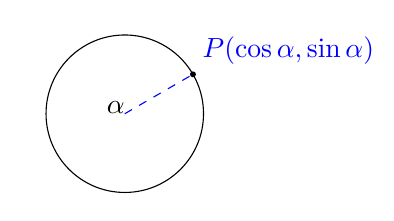
\begin{tikzpicture}		
		\tkzInit[xmax=2,ymax=2,xmin=-2,ymin=-2]
		\tkzGrid
		\tkzAxeXY
		
		\coordinate (A) at (1,0);
		\coordinate (O) at (0,0);
		\coordinate (P) at (0.866,0.5);
		\markangle[blue]{O}{P}{A}{0.5}{1.5}{$\alpha$}
		\draw[dashed, blue] (O) -- (P);	
		\filldraw (0.866,0.5) circle (0.03)
			node[blue, above right]{$P(\cos\alpha, \sin\alpha)$};
		\draw (0,0) circle (1);
	\end{tikzpicture}
\end{center}
Gi� nella figura identifichiamo le due funzioni fondamentali della goniometria: $\cos$ e $\sin$. Esse,
numericamente, rappresentano rispettivamente l'ascissa e l'ordinata del punto $P$ al variare di 
$\alpha$.\\
Seno e coseno non sono le uniche funzioni goniometriche, esistono infatti anche
\begin{align*}
\tan\alpha &= \frac{\sin\alpha}{\cos\alpha}\\
\cot\alpha &= \frac{1}{\tan\alpha}\\
\sec\alpha &= \frac{1}{\cos\alpha}\\
\csc\alpha &= \frac{1}{\sin\alpha}
\end{align*}
Da notare che spesso $\csc$ si trova anche scritto nella forma pi� estesa $\mathrm{cosec}$.\\
$\sin$ e $\cos$ rappresentano anche in un triangolo rettangolo
\begin{gather*}
	\cos\alpha = \frac{\text{Lunghezza cateto adiacente}}{\text{Lunghezza ipotenusa}}\\
	\sin\alpha = \frac{\text{Lunghezza cateto opposto}}{\text{Lunghezza ipotenusa}}
\end{gather*}
Per gli esercizi si vada \hyperref[ex:goniometria]{qui}.

\subsection{Angoli particolari}
Seno e coseno sono funzioni periodiche, ovvero che il loro valore sta all'interno di un insieme e si
ripete con un certo periodo.\\
Gli angoli particolari principali sono
\begin{alignat*}{2}
\sin\frac{\pi}{6} &= \frac{1}{2} &\qquad \cos\frac{\pi}{6} &= \frac{\sqrt{3}}{2}\\
\sin\frac{\pi}{4} &= \frac{\sqrt{2}}{2} & \cos\frac{\pi}{4} &= \frac{\sqrt{2}}{2}\\
\sin\frac{\pi}{3} &= \frac{\sqrt{3}}{2} & \cos\frac{\pi}{3} &= \frac{1}{2}
\end{alignat*}
Come si pu� notare ricordarli � piuttosto semplice: $\dfrac{\pi}{3}$ e $\dfrac{\pi}{6}$ sono gli 
angoli di un triangolo equilatero, $\dfrac{\pi}{4}$ � la diagonale di un quadrato.

\subsection{Relazione fondamentale}
La relazione fondamentale � quella che permetter� di trovare molte delle formule successive. Essa �
\begin{equation*}
\cos^2\alpha + \sin^2\alpha = 1
\end{equation*}

\subsection{Grafico delle funzioni}
\subsubsection{$\cos\alpha$}
\begin{center}
	\begin{tikzpicture}
		\tkzInit[xmin=-3.5,ymin=-1.5,xmax=3.5,ymax=1.5]
		\tkzGrid
		\tkzAxeXY
		\draw[red, thick, domain=-3.5:3.5, samples=500] plot({\x}, {cos(\x r)});
	\end{tikzpicture}
\end{center}
\subsubsection{$\sin\alpha$}
\begin{center}
	\begin{tikzpicture}
	\tkzInit[xmin=-3.5,ymin=-1.5,xmax=3.5,ymax=1.5]
	\tkzGrid
	\tkzAxeXY
	\draw[red, thick, domain=-3.5:3.5, samples=500] plot({\x}, {sin(\x r)});
	\end{tikzpicture}
\end{center}
\subsubsection{$\tan\alpha$}
\begin{center}
	\begin{tikzpicture}
	\tkzInit[xmin=-2,ymin=-2.5,xmax=2,ymax=2.5]
	\tkzGrid
	\tkzAxeXY
	\draw[red, thick, domain=-1.2:1.2, samples=500] plot({\x}, {tan(\x r)});
	\end{tikzpicture}
\end{center}

\subsection{Funzioni inverse}
Ovviamente se da un angolo possiamo ottenere un numero, possiamo fare anche il contrario. Per indicare
le funzioni inverse abbiamo due possibilit�
\begin{enumerate}
	\item Scrivere $f^{-1}(x)$
	\item Dare un nuovo nome alla funzione
\end{enumerate}

Nelle calcolatrici � molto pi� comune trovare $\sin^{-1}$ e gli altri per� non sono precisi e quindi
sarebbe da preferire $\arcsin$ o $\mathrm{asin}$ per brevit�. Il motivo � che se
\begin{equation*}
f:\;A\mapsto B,\,f^{-1}:\;B\mapsto A
\end{equation*}
per� per le funzioni goniometriche questo non accade infatti
\begin{equation*}
\sin x:\;\mathbb{R}\mapsto{[{-1},{+1}]} \qquad \cos x:\;\mathbb{R}\mapsto{[{-1},{1}]}
\end{equation*}
quando per�
\begin{equation*}
\arcsin x:\;{[{-1},{1}]}\mapsto{[{-\frac{\pi}{2}},{\frac{\pi}{2}}]} \quad 
\arccos:\;{[{-1},{1}]}\mapsto{[0,{\pi}]}
\end{equation*}
I grafici sono i seguenti
\subsubsection{$\arccos x$}
\begin{center}
	\begin{tikzpicture}
	\tkzInit[xmin=-2,ymin=-0.5,xmax=2,ymax=3]
	\tkzGrid
	\tkzAxeXY
	\draw[red, thick, domain=-1:1, samples=500] plot({\x}, {rad(acos(\x))});
	\end{tikzpicture}
\end{center}
\subsubsection{$\arcsin x$}
\begin{center}
	\begin{tikzpicture}
	\tkzInit[xmin=-2,ymin=-2,xmax=2,ymax=2]
	\tkzGrid
	\tkzAxeXY
	\draw[red, thick, domain=-1:1, samples=500] plot({\x}, {rad(asin(\x))});
	\end{tikzpicture}
\end{center}

\subsection{Formule goniometriche}
Le formule goniometriche permettono di pasare da una funzione ad un'altra. Una delle caratteristiche 
pi� importanti � l'esistenza dei cos� denominati \textbf{angoli associati}. Essi sono angoli 
particolari che assumono valori facili da scambiare e ricordare. Essi sono
\begin{alignat*}{2}
\cos(\pi\pm x) & = -\cos x &\qquad \cos(-x) &= \cos x\\
\sin(\pi\pm x) &= \mp\sin x & \sin(-x) &= -\sin x\\
\tan(\pi\pm x) &= \pm\tan x & \tan(-x) &= -\tan x
\end{alignat*}
In associazione a questi che sono i pi� comuni, sono anche presenti i seguenti
\begin{alignat*}{2}
\cos\left(\frac{\pi}{2}\pm x\right) &= \mp\sin x &\qquad \cos\left(\frac{3}{2}\pi\pm x\right) = 
\pm\sin x\\
\sin\left(\frac{\pi}{2}\pm x\right) &= \pm\cos x &\qquad \sin\left(\frac{3}{2}\pi\pm x\right) = 
-\cos x\\
\tan\left(\frac{\pi}{2}\pm x\right) &= \mp\cot x &\qquad \tan\left(\frac{3}{2}\pi\pm x\right) = 
\mp\cot x\\
\end{alignat*}
Si presti molta attenzione ai segni in quanto � molto facile confondersi.

\subsubsection{Addizione e sottrazione}
\begin{align*}
\cos(\gamma\pm\theta) &= \cos\gamma\cos\theta\mp\sin\gamma\sin\theta\\
\sin(\gamma\pm\theta) &= \sin\gamma\cos\theta\pm\cos\gamma\sin\theta\\
\tan(\gamma\pm\theta) &= \frac{\tan\gamma\pm\tan\theta}{1\mp\tan\gamma\tan\theta}
\end{align*}

\subsubsection{Duplicazione}
\begin{alignat*}{2}
\sin2x & =2\sin x\cos x &\qquad \cos2x &= \begin{cases}
\cos^2x - \sin^2x\\
1-2\sin^2x\\
2\cos^2x-1
\end{cases}\\
\tan2x &= \frac{2\tan x}{1-\tan^2x} & \cot2 &= \frac{\cot^2-1}{2\cot x}
\end{alignat*}

\subsubsection{Bisezione}
\begin{alignat*}{2}
\sin\frac{x}{2}&=\pm\sqrt{\frac{1-\cos x}{2}} &\qquad \cos\frac{x}{2}&=\pm\sqrt{\frac{1+\cos x}{2}}\\
\tan\frac{x}{2}&=\begin{dcases}
\frac{\sin x}{1+\cos x}\\
\frac{1-\cos x}{\sin x}
\end{dcases} & \cot\frac{x}{2} &= \begin{dcases}
\frac{1+\cos x}{\sin x}\\
\frac{\sin x}{1-\cos x}
\end{dcases}
\end{alignat*}
Il segno nella prima riga � da scegliersi $+$ se 
$\sin\frac{x}{2}\geq0\lor\cos\frac{x}{2}\geq0$, $-$ altrimenti.

\subsubsection{Parametriche}
Per queste formule poniamo
\begin{equation*}
t = \tan\frac{x}{2}
\end{equation*}
per comodit�.
\begin{alignat*}{2}
\sin x &= \frac{2t}{1+t^2} &\qquad \cos x &= \frac{1-t^2}{1+t^2}\\
\tan x &= \frac{2t}{1-t^2} & \cot x &= \frac{1-t^2}{2t}
\end{alignat*}

\subsubsection{Prostaferesi}
\begin{align*}
\sin p + \sin q &= 2\sin\frac{p+q}{2}\cos\frac{p-q}{2}\\
\sin p-\sin q &=2\cos\frac{p+q}{2}\sin\frac{p-q}{2}\\
\cos p+\cos q&=2\cos\frac{p+q}{2}\cos\frac{p-q}{2}\\
\cos p-\cos q&=-2\sin\frac{p+q}{q}\sin\frac{p-q}{2}
\end{align*}

\subsubsection{Werner}
\begin{align*}
\cos\gamma\cos\theta &= \frac{1}{2}[\cos(\gamma+\theta)+\cos(\gamma-\theta)]\\
\cos\gamma\sin\theta &= \frac{1}{2}[\sin(\gamma+\theta)-\sin(\gamma-\theta)]\\
\sin\gamma\sin\theta &= \frac{1}{2}[\cos(\gamma-\theta)-\cos(\gamma+\theta)]
\end{align*}

\subsection{Equazioni goniometriche}
Si definisce un'equazione goniometrica una qualsiasi equazione che abbia almeno una funzione 
goniometrica e che ha soluzioni solo per particolari angoli.
\subsubsection{$\sin x = m$}
\begin{equation*}
x = \arcsin m + 2k\pi \lor  x = \arcsin m +2k\pi-\pi
\end{equation*}

\subsubsection{$\cos x = m$}
\begin{equation*}
x = \pm\arccos m + 2k\pi
\end{equation*}

\subsubsection{$\tan x = m$}
\begin{equation*}
x = \arctan x + k\pi
\end{equation*}

\subsubsection{Equazioni lineari}
Le equazioni lineari vengono cos� definite perch� sono simili alla forma di una retta esplicita.
\begin{equation*}
a\sin x + b\cos x + c = 0
\end{equation*}
La risoluzione di questa pu� essere semplice per $b = 0 \lor a = 0$ in quanto si ritorna alle forme 
precedenti. Se invece $a\neq0 \land b\neq0$ si hanno due strade:
\begin{enumerate}
	\item metodo algebrico;
	\item metodo grafico;
\end{enumerate}
Il metodo algebrico � molto lungo e generalmente sconsigliato. In generale si sfrutta la 
parametrizzazione di $\sin$ e $\cos$ in $\tan \frac{x}{2}$.\\
Il metodo grafico consiste nel porre
\begin{equation*}
\cos x = X\,\text{ e } \sin x = Y
\end{equation*}
e poi risolvere il seguente sistema
\begin{equation*}
\begin{cases}
aY + bX + c = 0\\
X^2 + Y^2 = 1
\end{cases}
\end{equation*}

\subsubsection{Equazioni omogenee}
Si dicono omogenee se tutti i suoi elementi sono dello stesso grado. Per risolvere queste equazioni
in questa forma, abbiamo varie strade
\begin{itemize}
	\item Se \textbf{� presente il termine di grado $n$ in $\sin x$}, si divide tutto per 
	$\cos^nx\neq0$ ottenendo un'equazione di grado $n$ in $\tan x$ equivalente alla data;
	\item Se \textbf{� presente il termine di grado $n$ in $\cos x$}, si divide tutto per
	$\sin^nx\neq0$ ottenendo un'equazione di grado $n$ in $\cot x$ equivalente alla data;
	\item Se \textbf{nessuno dei precedenti � valido}, si raccolga a fattore comune;
\end{itemize}

\subsection{Teoremi sui triangoli}
\subsubsection{Area di un triangolo qualsiasi}
\begin{center}
	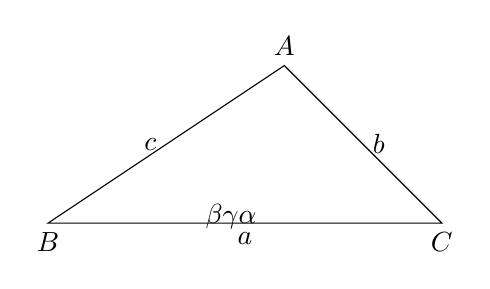
\begin{tikzpicture}
		\coordinate (A) at (1,2);
		\coordinate (B) at (-2,0);
		\coordinate (C) at (3,0);
		\draw (A) -- (B)
			node[pos=0.5,left]{$c$}
			node[pos=0,above]{$A$} -- (C)
			node[pos=0.5,below]{$a$}
			node[pos=0,below]{$B$} -- cycle
			node[pos=0.5,right]{$b$}
			node[pos=0,below]{$C$};
		\markangle{B}{A}{C}{0.3}{1.5}{$\beta$}
		\markangle[blue]{C}{B}{A}{0.3}{1.5}{$\gamma$}
		\markangle[orange]{A}{B}{C}{0.3}{2}{$\alpha$}
	\end{tikzpicture}
\end{center}
\begin{equation*}
\mathscr{A} = \frac{1}{2}ab\sin\gamma = \frac{1}{2}ac\sin\beta = \frac{1}{2}bc\sin\alpha
\end{equation*}

\subsubsection{Teorema della corda}
\begin{center}
	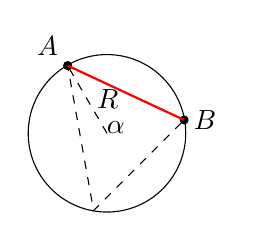
\begin{tikzpicture}
		\coordinate (A) at (-0.5,0.86);
		\coordinate (B) at (0.98,0.17);
		\coordinate (C) at (-0.17,-0.98);
		
		\draw (0,0) circle (1);
		\filldraw (A) circle (0.05)
			node[above left]{$A$};
		\filldraw (B) circle (0.05)
			node[right] {$B$};
		\draw[dashed] (A) -- (B) -- (C) -- cycle;
		\draw[thick,red] (A) -- (B);
		\draw[dashed] (0,0) -- (A)
			node[pos=0.5,right]{$R$};
		\markangle{C}{A}{B}{0.3}{1.5}{$\alpha$}
	\end{tikzpicture}
\end{center}
\begin{equation*}
\overline{AB} = 2R\sin\alpha
\end{equation*}

\subsubsection{Teorema dei seni}
\begin{center}
	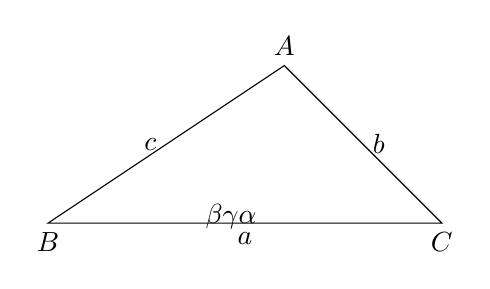
\begin{tikzpicture}
	\coordinate (A) at (1,2);
	\coordinate (B) at (-2,0);
	\coordinate (C) at (3,0);
	\draw (A) -- (B)
	node[pos=0.5,left]{$c$}
	node[pos=0,above]{$A$} -- (C)
	node[pos=0.5,below]{$a$}
	node[pos=0,below]{$B$} -- cycle
	node[pos=0.5,right]{$b$}
	node[pos=0,below]{$C$};
	\markangle{B}{A}{C}{0.3}{1.5}{$\beta$}
	\markangle[blue]{C}{B}{A}{0.3}{1.5}{$\gamma$}
	\markangle[orange]{A}{B}{C}{0.3}{2}{$\alpha$}
	\end{tikzpicture}
\end{center}
\begin{equation*}
\frac{a}{\sin\alpha} = \frac{b}{\sin\beta} = \frac{c}{\sin\gamma} = 2R
\end{equation*}

\subsubsection{Teoremi di Carnot}
\begin{center}
	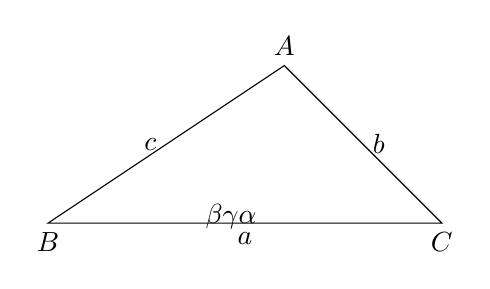
\begin{tikzpicture}
	\coordinate (A) at (1,2);
	\coordinate (B) at (-2,0);
	\coordinate (C) at (3,0);
	\draw (A) -- (B)
	node[pos=0.5,left]{$c$}
	node[pos=0,above]{$A$} -- (C)
	node[pos=0.5,below]{$a$}
	node[pos=0,below]{$B$} -- cycle
	node[pos=0.5,right]{$b$}
	node[pos=0,below]{$C$};
	\markangle{B}{A}{C}{0.3}{1.5}{$\beta$}
	\markangle[blue]{C}{B}{A}{0.3}{1.5}{$\gamma$}
	\markangle[orange]{A}{B}{C}{0.3}{2}{$\alpha$}
	\end{tikzpicture}
\end{center}
\begin{align*}
a^2 &= b^2+c^2-2bc\cos\alpha\\
b^2 &= a^2+c^2-2ac\cos\beta\\
c^2 &= a^2+b^2-2ab\cos\gamma
\end{align*}
